\chapter{Lec 01 - Rational Agents}
\section{Intelligent (or rational) agent}
An \textbf{agent} is anything that can be viewed as perceiving its environment through sensors and acting upon that environment through actuators. A human agent has eyes, ears, and other organs for sensors and hands, legs, vocal tract, and so on for actuators. A robotic agent might have cameras and infrared range finders for sensors and various motors for actuators. A software agent receives keystrokes, file contents, and network packets as sensory inputs and acts on the environment by displaying on the screen, writing files, and sending network packets.\newline\newline
In the context of the course, a \textbf{rational agent}, tries to achieve its goals as much as possible given the available information.\newline\newline
Mathematically speaking, we say that an agent’s behavior is described by the \textbf{agent function} that maps any given percept sequence to an action.
\[f : P^* \rightarrow A\]
Among all the classes of environments and tasks, we look for the agent (or class of agents) with the best performance. We can imagine tabulating the agent function that describes any given agent; for most agents, this would be a very large table, infinite, unless we place a bound on the length of percept sequences we want to consider. Computational limitations prevent the realization of perfect rationality.\newline\newline
Internally, the agent function for an artificial agent will be implemented by an \textbf{agent program}. It is important to keep these two ideas distinct. The agent function is an abstract mathematical description; the agent program is a concrete implementation, running within some physical system.\newline\newline
To illustrate these ideas, we use a very simple example, \textbf{the vacuum-cleaner world}: This particular world has just two locations: squares A and B. The vacuum agent perceives which square it is in and whether there is dirt in the square. It can choose to move left, move right, suck up the dirt, or do nothing. One very simple agent function is the following: if the current square is dirty, then suck; otherwise, move to the other square. This agent function can be represented as a table:
\begin{center}
    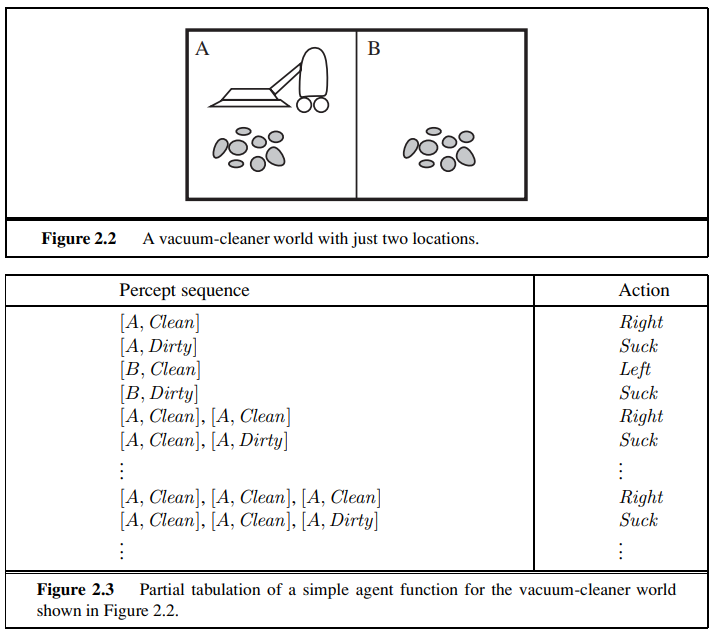
\includegraphics[]{images/Vacuum agent.png}
\end{center}
Various vacuum-world agents can be defined simply by filling in the right hand column in various ways. The obvious question, then, is this: What is the right way to fill out the table? 

\section{Rationality}
When an agent is plunked down in an environment, it generates a sequence of actions according to the percepts it receives. This sequence of actions causes the environment to go through a sequence of states. If the sequence is desirable, then the agent has performed well. This notion of \textbf{desirability} is captured by a \textbf{performance measure} that evaluates any given sequence of environment states. A \textbf{rational agent} chooses any action that maximizes the expected value of the performance measure given the sequence of perceptions obtained up to the current instant.\newline\newline
Obviously, there is not one fixed performance measure for all tasks and agents; typically, a designer will devise one appropriate to the circumstances:
\begin{itemize}
    \item +1 for each clean space in time $T$ ?
    \item +1 for each clean space per instant of time, -1 for movement ?
    \item ...
\end{itemize}
We need to be careful to distinguish between rationality and omniscience. An omniscient agent knows the actual outcome of its actions and can act accordingly; but omniscience is impossible in reality. Rationality maximizes expected performance, while perfection maximizes actual performance. A rational agent should be able to \textbf{gather information} (exploration), \textbf{learn} as much as possible from what it perceives and be \textbf{autonomous}.

\section{PEAS}
What is rational at any given time depends on four things:
\begin{itemize}
    \item The performance measure that defines the criterion of success.
    \item The agent’s prior knowledge of the environment.

    \item The actions that the agent can perform.

    \item The agent’s percept sequence to date.
\end{itemize}
Therefore, in designing an agent, we had to specify the performance measure, the environment, and the agent’s actuators and sensors. We group all these under the heading of the \textbf{task environment}. For the acronymically minded, we call this the \textbf{PEAS} (Performance, Environment, Actuators, Sensors) description. In designing an agent, the first step must always be to specify the task environment as fully as possible.\newline\newline
Consider, for example, the task of designing an automated taxi:
\begin{center}
    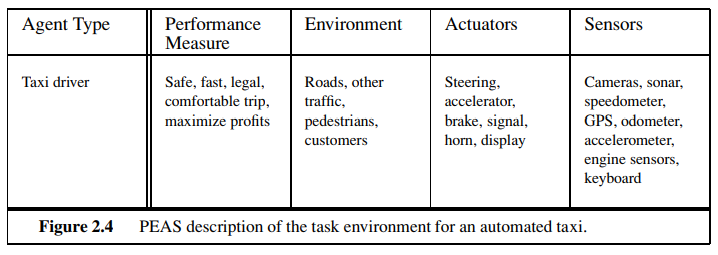
\includegraphics[]{images/Autonomous driving.png}
\end{center}

\subsection{Tasks environments}
The range of task environments that might arise in AI is obviously vast. We can, however, identify a fairly small number of dimensions along which task environments can be categorized:
\begin{itemize}
    \item \textbf{Fully observable} vs. \textbf{partially observable}: Whether an agent’s sensors give it access to the complete state of the environment at each point in time or not.

    \item \textbf{Single agent} vs. \textbf{multiagent}

    \item \textbf{Deterministic} vs. \textbf{stochastic}: Whether the next state of the environment is completely determined by the current state and the action executed by the agent or not.

    \item \textbf{Episodic} vs. \textbf{sequential}: In an episodic task environment, the agent’s experience is divided into atomic episodes. In each episode the agent receives a percept and then performs a single action. Crucially, the next episode \textbf{does not} depend on the actions taken in previous episodes. Many classification tasks are episodic. In sequential environments, on the other hand, the current decision could affect all future decisions. Chess and taxi driving are sequential.

    \item \textbf{Static} vs. \textbf{dynamic}: If the environment can change while an agent is deliberating, then we say the environment is dynamic for that agent; otherwise, it is static. Static environments are easy to deal with because the agent need not keep looking at the world while it is deciding on an action, nor need it worry about the passage of time. Dynamic environments, on the other hand, are continuously asking the agent what it wants to do; if it hasn’t decided yet, that counts as deciding to do nothing.

    \item \textbf{Discrete} vs. \textbf{continuous}: The discrete/continuous distinction applies to the state of the environment, to the way time is handled, and to the percepts and actions of the agent. For example, the chess environment has a finite number of distinct states (excluding the clock). Chess also has a discrete set of percepts and actions. Taxi driving is a continuous-state and continuous-time problem.  Input from digital cameras is discrete, strictly speaking, but is typically treated as representing continuously varying intensities and locations.

    \item \textbf{Known} vs. \textbf{unknown}:  In a known environment, the outcomes (or outcome probabilities if the environment is stochastic) for all actions are given. Obviously, if the environment is unknown, the agent will have to learn how it works in order to make good decisions. Note that the distinction between known and unknown environments is not the same as the one between fully and partially observable environments.  It is quite possible for a known environment to be partially observable; for example, in solitaire card games, I know the rules but am still unable to see the cards that have not yet been turned over. Conversely, an unknown environment can be fully observable—in a new video game, the screen may show the entire game state but I still don’t know what the buttons do until I try them.
\end{itemize}
\begin{center}
    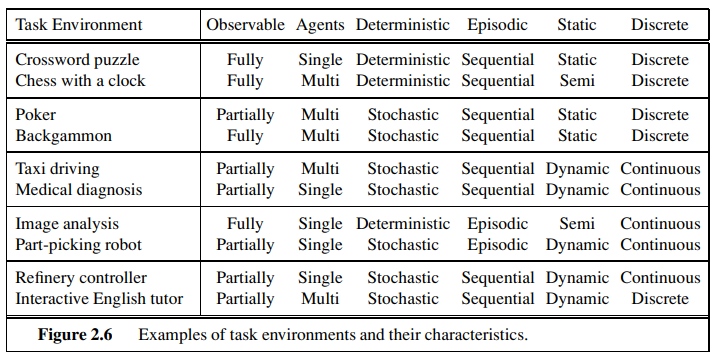
\includegraphics[]{images/tasks environment.png}
\end{center}
The type of environment largely determines the design of the agent. The real world is, of course, partially observable, stochastic, sequential, dynamic, continuous, multi-agent.

\section{The Structure of Agents}
The job of AI is to design an agent program that implements the agent function, the mapping from percepts to actions. We assume this program will run on some sort of computing device with physical sensors and actuators. We call this \textbf{the architecture}:
\[agent = architecture + program\]
Obviously, the program we choose has to be one that is appropriate for the architecture. If the program is going to recommend actions like Walk, the architecture had better have legs. The architecture might be just an ordinary PC.

\subsection{Agent programs}
The agent programs that we'll design have the same skeleton: they take the current percept as input from the sensors and return an action to the actuators. We can design a table-driven agent as follows:
\begin{center}
    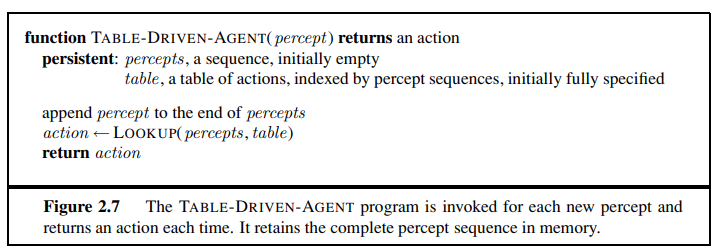
\includegraphics[]{images/Table-driven agent.png}
\end{center}
The key challenge for AI is to find out how to write programs that, to the extent possible, produce rational behavior from a smallish program rather than from a vast table.\newline\newline
Four kinds of agents can be defined in general:
\begin{itemize}
    \item Simple reflex agents;
    \item Model-based reflex agents;
    \item Goal-based agents; and
    \item Utility-based agents
\end{itemize}
They differ in the internal components they use to generate actions. All these types of agents can be made into agents who learn.

\subsubsection{Simple reflex agents}
The simplest kind of agent is the simple reflex agent. These agents select actions on the basis of the current percept, ignoring the rest of the percept history. Their behavior is defined by a set of condition-action rules, for example, \textbf{if} car-in-front-is-braking \textbf{then} initiate-braking. One example of this kind of agent is the vacuum-agent presented before.\newline\newline
Simple reflex agents have the admirable property of being simple, but they turn out to be of limited intelligence. If the environment is partially observable it can fail.

\subsubsection{Model-based reflex agents}
The most effective way to handle partial observability is for the agent to keep track of the part of the world it can’t see now. That is, the agent should maintain some sort of \textbf{internal state} that depends on the percept history and thereby reflects at least some of the unobserved aspects of the current state.\newline\newline
Updating this internal state information as time goes by requires two kinds of knowledge to be encoded in the agent program.  First, we need some information about how the world evolves independently of the agent.  Second, we need some information about how the agent’s own actions affect the world. This knowledge about “how the world works" is called a \textbf{model} of the world. An agent that uses such a model is called a \textbf{model-based agent}.  For example, an automated taxi may not be able to see around the large truck that has stopped in front of it and can only guess about what may be causing the hold-up. Thus, uncertainty about the current state may be unavoidable, but the agent still has to make a decision.

\subsubsection{Goal-based agents}
Knowing something about the current state of the environment is not always enough to decide what to do. For example, at a road junction, the taxi can turn left, turn right, or go straight on. In other words, as well as a current state description, the agent needs some sort of goal information that describes situations that are desirable, for example, being at the passenger’s destination.  The agent program can combine this with the model to choose actions that achieve the goal.\newline\newline
Goal-based agents are more \textbf{flexible} because they can automatically adapt their relevant behaviors to suit new conditions. For example, If it starts to rain, the agent can update its knowledge of how effectively its brakes will operate. For the reflex agent, on the other hand, we would have to rewrite many condition–action rules.

\subsubsection{Utility-based agents}
Goals alone are not enough to generate high-quality behavior in most environments.  For example, many action sequences will get the taxi to its destination (thereby achieving the goal) but some are quicker, safer, more reliable, or cheaper than others.  Goals just provide a crude binary distinction between “happy” and “unhappy” states. A more general performance measure should allow a comparison of different world states according to exactly how happy
they would make the agent.\newline\newline
We have already seen that a performance measure assigns a score to any given sequence of environment states, so it can easily distinguish between more and less desirable ways of getting to the taxi’s destination.  An agent’s \textbf{utility function} is essentially an internalization of the performance measure. If the internal utility function and the external performance easure are in agreement, then an agent that chooses actions to maximize its utility will be rational according to the external performance measure.\newline\newline
Like goal-based agents, a utility-based agent has many advantages in
terms of flexibility and learning.\newline\newline
Furthermore, in two kinds of cases, goals are inadequate but
a utility-based agent can still make rational decisions. First, when there are conflicting goals, only some of which can be achieved (for example, speed and safety), the utility function specifies the appropriate \textbf{tradeoff}. Second, when there are several goals that the agent can aim for, none of which can be achieved with certainty, utility provides a way in which the likelihood of success can be weighed against the importance of the goals.

\subsubsection{Learning agents}
We have described agent programs with various methods for selecting actions. We have not, so far, explained how the agent programs come into being.
\begin{center}
    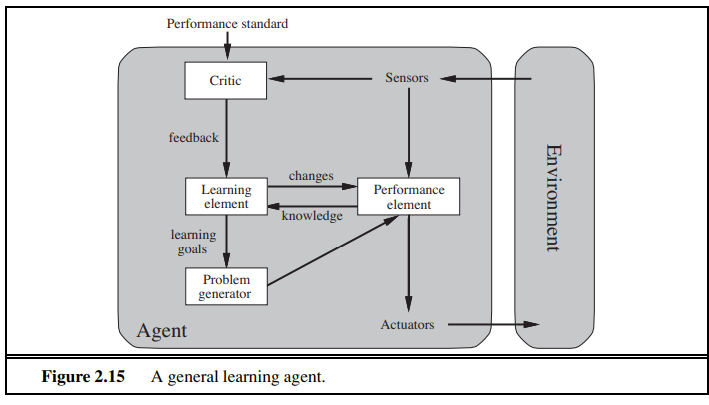
\includegraphics[]{images/Learning agent.png}
\end{center}
A learning agent can be divided into four conceptual components. The most important distinction is between the \textbf{learning element}, which is responsible for making improvements, and the \textbf{performance element}, which is responsible for electing external actions. The performance element is what we have previously considered to be the entire agent: it takes in percepts and decides on actions. The learning element uses
feedback from the \textbf{critic} on how the agent is doing and determines how the performance element should be modified to do better in the future. The critic tells the learning element how well the agent is doing with respect to a fixed performance standard. The last component of the learning agent is the \textbf{problem generator}. It is responsible for suggesting actions that will lead to new and informative experiences. Basically, it is necessary to improve the generalization of the agent's behaviors.

\subsubsection{Representing the environment}
We can place the environment representations along an axis of increasing complexity and expressive power: \textbf{atomic}, \textbf{factored}, and \textbf{structured}.
\begin{center}
    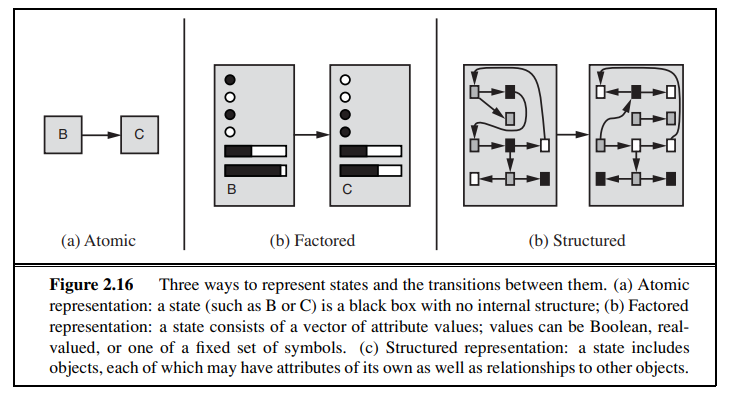
\includegraphics[]{images/environment repr.png}
\end{center}
\begin{itemize}
    \item In an \textbf{atomic representation} each state of the world is indivisible.

    \item \textbf{factored representation}: splits up each state into a fixed set of variables or attributes, each of which can have a value.

    \item \textbf{structured representation}: in which objects and their various and varying relationships can be described explicitly
\end{itemize}
